% UCL Thesis LaTeX Template
%  (c) Ian Kirker, 2014
% 
% This is a template/skeleton for PhD/MPhil/MRes theses.
%
% It uses a rather split-up file structure because this tends to
%  work well for large, complex documents.
% We suggest using one file per chapter, but you may wish to use more
%  or fewer separate files than that.
% We've also separated out various bits of configuration into their
%  own files, to keep everything neat.
% Note that the \input command just streams in whatever file you give
%  it, while the \include command adds a page break, and does some
%  extra organisation to make compilation faster. Note that you can't
%  use \include inside an \include-d file.
% We suggest using \input for settings and configuration files that
%  you always want to use, and \include for each section of content.
% If you do that, it also means you can use the \includeonly statement
%  to only compile up the section you're currently interested in.
% You might also want to put figures into their own files to be \input.

% For more information on \input and \include, see:
%  http://tex.stackexchange.com/questions/246/when-should-i-use-input-vs-include


% Formatting rules for theses are here: 
%  http://www.ucl.ac.uk/current-students/research_degrees/thesis_formatting
% Binding and submitting guidelines are here:
%  http://www.ucl.ac.uk/current-students/research_degrees/thesis_binding_submission

% This package goes first and foremost, because it checks all 
%  your syntax for mistakes and some old-fashioned LaTeX commands.
% Note that normally you should load your documentclass before 
%  packages, because some packages change behaviour based on
%  your document settings.
% Also, for those confused by the RequirePackage here vs usepackage
%  elsewhere, usepackage cannot be used before the documentclass
%  command, while RequirePackage can. That's the only functional
%  difference.
\RequirePackage[l2tabu, orthodox]{nag}


% ------ Main document class specification ------
% The draft option here prevents images being inserted,
%  and adds chunky black bars to boxes that are exceeding 
%  the page width (to show that they are).
% The oneside option can optionally be replaced by twoside if
%  you intend to print double-sided. Note that this is
%  *specifically permitted* by the UCL thesis formatting
%  guidelines.
%
% Valid options in terms of type are:
%  phd
%  mres
%  mphil
%\documentclass[12pt,phd,draft,a4paper,oneside]{ucl_thesis}
\documentclass[12pt,phd,a4paper,oneside]{ucl_thesis}


% Package configuration:
%  LaTeX uses "packages" to add extra commands and features.
%  There are quite a few useful ones, so we've put them in a 
%   separate file.
% -------- Packages --------

% This package just gives you a quick way to dump in some sample text.
% You can remove it -- it's just here for the examples.
\usepackage{blindtext}

% This package means empty pages (pages with no text) won't get stuff
%  like chapter names at the top of the page. It's mostly cosmetic.
\usepackage{emptypage}

% The graphicx package adds the \includegraphics command,
%  which is your basic command for adding a picture.
\usepackage{graphicx}

% This command is provided by the graphicx package, and 
%  controls the default dpi resolution of images you use.
%  72 is the default, but 300 is more normal, and 600 is
%  as good as you can expect to be able to get on normal paper.
\pdfimageresolution=300


% The float package improves LaTeX's handling of floats,
%  and also adds the option to *force* LaTeX to put the float
%  HERE, with the [H] option to the float environment.
\usepackage{float}

% The amsmath package enhances the various ways of including
%  maths, including adding the align environment for aligned
%  equations.
\usepackage{amsmath}

% Use these two packages together -- they define symbols
%  for e.g. units that you can use in both text and math mode.
\usepackage{gensymb}
\usepackage{textcomp}
% You may also want the units package for making little
%  fractions for unit specifications.
%\usepackage{units}


% The setspace package lets you use 1.5-sized or double line spacing.
\usepackage{setspace}
\setstretch{1.5}

% That just does body text -- if you want to expand *everything*,
%  including footnotes and tables, use this instead:
%\renewcommand{\baselinestretch}{1.5}


% PGFPlots is either a really clunky or really good way to add graphs
%  into your document, depending on your point of view.
% There's waaaaay too much information on using this to cover here,
%  so, you might want to start here:
%   http://pgfplots.sourceforge.net/
%  or here:
%   http://pgfplots.sourceforge.net/pgfplots.pdf
%\usepackage{pgfplots}
%\pgfplotsset{compat=1.3} % <- this fixed axis labels in the version I was using

% PGFPlotsTable can help you make tables a little more easily than
%  usual in LaTeX.
% If you're going to have to paste data in a lot, I'd suggest using it.
%  You might want to start with the manual, here:
%  http://pgfplots.sourceforge.net/pgfplotstable.pdf
%\usepackage{pgfplotstable}

% These settings are also recommended for using with pgfplotstable.
%\pgfplotstableset{
%	% these columns/<colname>/.style={<options>} things define a style
%	% which applies to <colname> only.
%	empty cells with={--}, % replace empty cells with '--'
%	every head row/.style={before row=\toprule,after row=\midrule},
%	every last row/.style={after row=\bottomrule}
%}


% The mhchem package provides chemistry formula typesetting commands
%  e.g. \ce{H2O}
%\usepackage[version=3]{mhchem}

% And the chemfig package gives a weird command for adding Lewis 
%  diagrams, for e.g. organic molecules
%\usepackage{chemfig}

% The linenumbers command from the lineno package adds line numbers
%  alongside your text that can be useful for discussing edits 
%  in drafts.
% Remove or comment out the command for proper versions.
%\usepackage[modulo]{lineno}
% \linenumbers 


% Alternatively, you can use the ifdraft package to let you add
%  commands that will only be used in draft versions
%\usepackage{ifdraft}

% For example, the following adds a watermark if the draft mode is on.
%\ifdraft{
%  \usepackage{draftwatermark}
%  \SetWatermarkText{\shortstack{\textsc{Draft Mode}\\ \strut \\ \strut \\ \strut}}
%  \SetWatermarkScale{0.5}
%  \SetWatermarkAngle{90}
%}


% The multirow package adds the option to make cells span 
%  rows in tables.
\usepackage{multirow}


% Subfig allows you to create figures within figures, to, for example,
%  make a single figure with 4 individually labeled and referenceable
%  sub-figures.
% It's quite fiddly to use, so check the documentation.
%\usepackage{subfig}

% The natbib package allows book-type citations commonly used in
%  longer works, and less commonly in science articles (IME).
% e.g. (Saucer et al., 1993) rather than [1]
% More details are here: http://merkel.zoneo.net/Latex/natbib.php
%\usepackage{natbib}

% The bibentry package (along with the \nobibliography* command)
%  allows putting full reference lines inline.
%  See: 
%   http://tex.stackexchange.com/questions/2905/how-can-i-list-references-from-bibtex-file-in-line-with-commentary
\usepackage{bibentry} 

% The isorot package allows you to put things sideways 
%  (or indeed, at any angle) on a page.
% This can be useful for wide graphs or other figures.
%\usepackage{isorot}

% The caption package adds more options for caption formatting.
% This set-up makes hanging labels, makes the caption text smaller
%  than the body text, and makes the label bold.
% Highly recommended.
\usepackage[format=hang,font=small,labelfont=bf]{caption}

% If you're getting into defining your own commands, you might want
%  to check out the etoolbox package -- it defines a few commands
%  that can make it easier to make commands robust.
\usepackage{etoolbox}

%twoside for double page printing
\usepackage{graphics}
\usepackage{graphicx}
%\usepackage[lined,boxed,commentsnumbered]{algorithm2e}
\usepackage{paralist}
\usepackage{amssymb}
\usepackage{amstext}
\usepackage{amsmath}
\usepackage{amsthm}
\usepackage{algorithm}
\usepackage{algorithmic}
\usepackage{multirow}
\usepackage{url}
\usepackage[table]{xcolor}
\usepackage{pdflscape}
\usepackage{rotating}
\usepackage{tikz}
%\usepackage{natbib}
\usepackage{afterpage}

\makeatletter
\newenvironment{subtheorem}[1]{%
	\def\subtheoremcounter{#1}%
	\refstepcounter{#1}%
	\protected@edef\theparentnumber{\csname the#1\endcsname}%
	\setcounter{parentnumber}{\value{#1}}%
	\setcounter{#1}{0}%
	\expandafter\def\csname the#1\endcsname{\theparentnumber.\Alph{#1}}%
	\ignorespaces
}{%
\setcounter{\subtheoremcounter}{\value{parentnumber}}%
\ignorespacesafterend
}

\newtheorem{mydef}{Definition}
\newtheorem{fact}{Fact}
\newtheorem{myAssumption}{Assumption}
\newtheorem{myequ}{Equation}
\newcounter{parentnumber}
\newtheorem{example}{Example}
\newtheorem{lemma}{Proposition}
\newtheorem{conj}[subsubsection]{Conjecture}{\bfseries}{\rmfamily}



% Sets up links within your document, for e.g. contents page entries
%  and references, and also PDF metadata.
% You should edit this!
%%
%% This file uses the hyperref package to make your thesis have metadata embedded in the PDF, 
%%  and also adds links to be able to click on references and contents page entries to go to 
%%  the pages.
%%

% Some hacks are necessary to make bibentry and hyperref play nicely.
% See: http://tex.stackexchange.com/questions/65348/clash-between-bibentry-and-hyperref-with-bibstyle-elsart-harv
\usepackage{bibentry}
\makeatletter\let\saved@bibitem\@bibitem\makeatother
\usepackage[pdftex,hidelinks]{hyperref}
\makeatletter\let\@bibitem\saved@bibitem\makeatother
\makeatletter
\AtBeginDocument{
    \hypersetup{
        pdfsubject={Thesis Subject},
        pdfkeywords={Thesis Keywords},
        pdfauthor={Author},
        pdftitle={Title},
    }
}
\makeatother
    


% And then some settings in separate files.
% These settings are from:
%  http://mintaka.sdsu.edu/GF/bibliog/latex/floats.html

% They give LaTeX more options on where to put your figures, and may
%  mean that fewer of your figures end up at the tops of pages far
%  away from the thing they're related to.

% Alters some LaTeX defaults for better treatment of figures:
% See p.105 of "TeX Unbound" for suggested values.
% See pp. 199-200 of Lamport's "LaTeX" book for details.

%   General parameters, for ALL pages:
\renewcommand{\topfraction}{0.9}	% max fraction of floats at top
\renewcommand{\bottomfraction}{0.8}	% max fraction of floats at bottom

%   Parameters for TEXT pages (not float pages):
\setcounter{topnumber}{2}
\setcounter{bottomnumber}{2}
\setcounter{totalnumber}{4}     % 2 may work better
\setcounter{dbltopnumber}{2}    % for 2-column pages
\renewcommand{\dbltopfraction}{0.9}	% fit big float above 2-col. text
\renewcommand{\textfraction}{0.07}	% allow minimal text w. figs

%   Parameters for FLOAT pages (not text pages):
\renewcommand{\floatpagefraction}{0.7}	% require fuller float pages
% N.B.: floatpagefraction MUST be less than topfraction !!
\renewcommand{\dblfloatpagefraction}{0.7}	% require fuller float pages

% remember to use [htp] or [htpb] for placement,
% e.g. 
%  \begin{figure}[htp]
%   ...
%  \end{figure} % For things like figures and tables
\bibliographystyle{unsrt}   % For bibliographies

% Title Settings
\setcounter{secnumdepth}{3}
\setcounter{tocdepth}{3}
\title{A Thesis Title}
\author{Author Name}
\department{Department of Something}


\begin{document}



\nobibliography*
% This is a dumb trick that works with the bibentry package to let
%  you put bibliography entries whereever you like.
% I used this to put references to papers a chapter's work was 
%  published in at the end of that chapter.
% For more information, see: http://stefaanlippens.net/bibentry

% If you haven't finished making your full BibTex file yet, you
%  might find this useful -- it'll just replace all your
%  citations with little superscript notes.
% Uncomment to use.
%\renewcommand{\cite}[1]{\emph{\textsuperscript{[#1]}}}

% At last, content! Remember filenames are case-sensitive and 
%  *must not* include spaces.
\maketitle
\makedeclaration

\begin{abstract} % 300 word limit
In this thesis we study two major topics in cryptanalysis and optimization: software algebraic cryptanalysis and elliptic curve optimizations in cryptanalysis. The idea of algebraic cryptanalysis is to model a cipher by a Multivariate Quadratic (MQ) equation system. Solving MQ is an NP-hard problem. However, NP-hard problems have a point of phase transition where the problems become easy to solve. This thesis explores different optimizations to make solving algebraic cryptanalysis problems easier. 

We first worked on guessing a well-chosen number of key bits, a specific optimization problem leading to guess-then-solve attacks on GOST cipher. In addition to attacks, we propose two new security metrics of contradiction immunity and SAT immunity applicable to any cipher. These optimizations play a pivotal role in recent highly competitive results on full GOST. This and another cipher Simon, which we cryptanalyzed were submitted to ISO to become a global encryption standard which is the reason why we study the security of these ciphers in a lot of detail. 

Another optimization direction is to use well-selected data in conjunction with Plaintext/Ciphertext pairs following a truncated differential property. These allow to supplement an algebraic attack with extra equations and reduce solving time. This was a key innovation in our algebraic cryptanalysis work on NSA block cipher Simon and we could break up to 10 rounds of Simon64/128. The second major direction in our work is to inspect, analyse and predict the behaviour of ElimLin attack the complexity of which is very poorly understood, at a level of detail never seen before. Our aim is to extrapolate and discover the limits of such attacks, and go beyond with several types of concrete improvement. 

Finally, we have studied some optimization problems in elliptic curves which also deal with polynomial arithmetic over finite fields. We have studied existing implementations of the secp256k1 elliptic curve which is used in many popular cryptocurrency systems such as Bitcoin and we introduce an optimized attack on Bitcoin brain wallets and improved the state of art attack by 2.5 times. 

\vskip5pt
\vskip5pt
{\bf Keywords:} algebraic cryptanalysis, SAT solver, ElimLin, symmetric encryption,  GOST, Simon, Bitcoin brain wallets, Elliptic curves
\end{abstract}

\begin{impactstatement}
	This thesis aims to make both acdemic and non acdemic research impacts. We aim to make contribution to the reasearch area in algebraic cryptanalysis. We proposed a few methods to improve algebraic attack, such as using well selected plaintext ciphertext pairs, guessing a selected set of key bits. We studied fisrt time in detail how ElimLin algorithm works and developed tools for analysising newly generated linear equations. 
	
	Our proposed methods are preformed on well known or widely used ciphers: Russian GOST cipher and new NSA block cipher SIMON. Both of them has been submitted to ISO in order to become an international standard. As an impact of our research, together with other people's research work, ISO rejected both of the ciphers.
	
	We also studied the security of Bitcoin brain wallets, and published a brainwallet attack which improved the state of art by a factor of 2.5. Our work has been reported by a number of tech websites, also widely read within Bitcoin community. We made Bitcoin brain wallets users relise it's not a secure way to store their money. As a result, Brainwallet.org, the website which are used by Bitcoin comunity to generate brain wallets has permenantly closed.
	
\end{impactstatement}

\begin{acknowledgements}
I would like to express my sincere gratitude to my supervisor Dr. Nicolas Courtois for his guidance and advice throughout my research. He is an excellent example of codebreaker and a great mentor.  His patience, motivation, enthusiasm and immense knowledge have been invaluable throughout my academic and personal development.

I would like to express my great appreciation to Dr. Daniel Hulme for his endless support, continuous encouragement, valuable suggestions and the working opportunity he offered from Satalia over the years. Furthermore, I thank my UCL colleagues Dr. Theodosis Mourouzis, Dr. Jie Xiong and Yongxin Yang for the sleepless nights when we were working together before deadlines, and for all the fun we have had in the last few years.

I extend my gratitude to Dr. Mark Herbster, Dr. David Clark, Dr. Earl Barr from UCL and Steven Poulson from Cisco, for their kindness and advice, offering internship opportunities in their groups and leading me in working on exciting projects. 

Finally, and most importantly, a very special thank you goes to my parents and my wife for their love during all these years of my Ph.D. studies. It would have been impossible to have done it without them.

\end{acknowledgements}

\setcounter{tocdepth}{2} 
% Setting this higher means you get contents entries for
%  more minor section headers.

\tableofcontents
\listoffigures
\listoftables


\chapter{Introduction}
\label{chapterlabel1}

Cryptography is the study of mathematical techniques that ensure the confidentiality and integrity of information. Cryptography is one of the oldest fields of technical study which we can find records of. Going back to 1900 BC,  cryptography is found in non-standard hieroglyphs carved into monuments from the Old Kingdom of Egypt \cite{kahn1996codebreakers}. Modern cryptography started out as classified military technology, but now has become very common in our daily lives. Cryptography is not only used in banking cards, secure websites and electronic signatures, but also in public transport cards, car keys, and building passes. 

Block cipher is one of the main tools in cryptography; It uses a secret key to transform a plaintext into a ciphertext in such a way that this secret key is needed to recover the original plaintext. During the last 30 years, the academic research on the security of block ciphers has evolved from an empirical way to solve the problem of designing a secure algorithm towards a list of well-understood and well-established  security properties that a block cipher must fulfil in order to be secure. Unfortunately, the  security of a block cipher is still heavily dependent on the talent, the intuition, and the time at disposal of the people attempting to break it!

Currently, because of the continuously growing impact of mobile phones, smart cards, RFID tags, sensor networks, and the rapid development in the Internet of Things (IoT), there is a huge demand to provide security and to design suitable cryptographic algorithms that can be efficiently implemented in resource-constrained devices. The area of cryptography that studies the design and the security of such lightweight cryptographic primitives, called lightweight cryptography, is rapidly evolving and becoming increasingly important. 

Most of the cryptographic primitives have been carefully designed, especially those that have been standardized. However, not all of them have been well studied by researchers. Special properties  inside widely used cryptography schemes, which might lead to faster attacks, are discovered every year. Also, in real life cryptography applications, bad design, implementation or choice of parameters could lead to huge security issues.

The main aim of my PhD research is to investigate the use of and to develop various optimization tools and software, such as SAT solver and evolutionary algorithms, in the field of automated cryptanalysis; apply cryptanalysis techniques to modern block ciphers, (such as GOST\cite{gost198928147}, Simon \cite{NSAciphers} and even elliptic curve cryptography problems) with optimization tools or software; and check if such tools can improve the current best attacks and discover new attacks. We hope to contribute to future government standards and popular cryptography applications. In this thesis, our cryptanalysis targets are the Russian government standard cipher GOST, the NSA newly proposed cipher Simon, and Bitcoin Elliptic Curve.

The first part of this thesis focuses on software algebraic crytanalysis. Automated “black box” techniques, such as SAT solvers or Gr\"{o}bner basis computations, have become increasingly sophisticated and powerful. In the domain of algebraic cryptanalysis, they are used to solve equation systems that are converted from the cipher. Solving such equation systems is an NP-hard problem. When the problem becomes larger (e.g., trying to solve a larger number%numbers
 of rounds), it becomes impossible to solve using a normal PC. This is the fundamental problem of software algebraic cryptanalysis. However, NP-hard problems normally have a ``phase transition" point when the problem is suddenly changed from ``hard to solve" to ``easy to solve". This phase transition also appears in software algebraic cryptanalysis, for example, using chosen plaintext in a counter mode then solving by ElimLin \cite{ElimLinR}. In this thesis, we explore different ways to improve software algebraic cryptanalysis. We introduce two possible directions: guessing a set of well chosen key bits and using well-chosen samples. We study GOST and Simon for a concrete number of rounds, discover properties inside the cipher structure which will lead to more efficient attacks. We will then demonstrate how to make these attacks work better by: %In this thesis, all solving algorithms are kept as black box. 
% inspection: learn what is trival and non-travil behavior of ElimLin algorithm by inspecting the equations found by ElimLin, prediction: predict when ElimLin algorithm will terminate and solve the problem, interpolation Selection of samples / key bits: combining other cryanalysis ideas (such as truncated differential attack and cube attack) study how selected samples / key bits make the problem become easy to solve

\begin{itemize}
	\item \textbf{Inspection}: Learn what is trivial and non-trivial behavior of ElimLin algorithm by inspecting the equations found by ElimLin.
	\item \textbf{Prediction and interpolation}: Predict when the ElimLin algorithm will terminate and solve the problem.
	\item \textbf{Guess-then-solve}: With some ``cost of guessing'', we can reduce the solving complexity. Selecting the right set of bits to guess makes the problem easier to solve.
	\item \textbf{Selection of samples}: Use specific plaintexts suggested by independent well-known attacks,
	such as [generalized] linear attacks, truncated differential properties and cube attacks.
\end{itemize}

The second part of this thesis is about understanding how elliptic curve cryptography can be efficiently coded for fast implementation and also cryptanalysis. We discussed an open research problem for solving Elliptic Curve Discrete Logarithm Problem and also implemented a dedicated speed optimization for Bitcoin brain wallet attack. Bitcoin is a cryptocurrency that was invented in 2008 and has become extremely popular since 2012. Bitcoin users can deterministically derive the private key used for transmitting money from a password. Such wallets are known as brain wallets. Brain wallets are appealing because they free users from storing their private keys. Unfortunately, brain wallets were not designed carefully enough and allowed attackers to conduct unlimited offline password guessing. In 2015, a white hat hacker published the implementation of the brain wallet attack. The results of this attack were later published in 2016 \cite{vasek2016bitcoin}. We believe that such an attack can be made faster to make brain wallets much more vulnerable. In order to optimize the attack, we study Elliptic Curve secp256k1, which is used in Bitcoin. We focus on the speed of the key generation process and provide the first detailed benchmarks for all the major implementations of this curve. The key generation process is a fundamental part in the Bitcoin brain wallet attack, which is also the most part cost most time to compute. Our optimized attack improves the state-of-art by a factor of 2.5 in private key checking speed.
%Here I listed three research problems which I investigate inside my PhD research:

%1. Explore how software and tools can be used (and potentially develop such a tool) in the field of automated cryptanalysis, especially in SAT solvers used in algebraic attack. 

%Automated “black box” techniques, such as SAT solvers or Grobner basis computations, have become increasingly sophisticated and powerful. In the domain of algebraic cryptanalysis, they are used to attack cryptosystems. But what is the limitation of this kind of attacks and how the current methods can be improved?

%2. Study Russian government standard cipher GOST, NSA newly proposed cipher SIMON, and Semaev cipher (described in section \ref{sec:summationPoly})  for a concrete number of rounds, discover properties inside the cipher structure which will lead to more efficient attacks

%Carefully study the structure of the cipher and try to find special properties which could lead to a faster attack. Combined automated tools and make use of other cryptanalysis techniques to improve current best attack.  

%3. Study elliptic curves with special properties, identify possible attacks and implementation improvements.
%\section{Structure of the Thesis}

%\section{My Publications}
%Some of the results presented in this thesis were published in the following conferences and journals:

\chapter{My First Content Chapter}
\label{chapterlabel2}

% This just dumps some pseudolatin in so you can see some text in place.
\blindtext

\chapter{Cryptanalysis of Block Ciphers} \label{ch:CoBC}
\label{Cryptanalysis of block ciphers}
%\input{method}
The history of cryptanalysis is as long and as fascinating as the history of cryptography. For example, in 1917, an article in ``Scientific American" claimed that the Vigen\`{e}re cipher was ``impossible of translation" \cite{knudsen1998block}. Today, most cryptography classes at university use the Vigen\`{e}re cipher as an exercise to illustrate that this claim is not true. When discussing the security of a cryptosystem, one needs to define a model that works in the real world for which we will use the model of Shannon \cite{shannon1949communication}.

%TO DO 插图 

The sender and the receiver share a common key $K$ over a secure channel in advance. The sender encrypts a plaintext P using the secret key $K$, sends ciphertext C over an insecure channel to the receiver. The receiver then decrypts C to P using K. The attacker has access to the insecure channel and can intercept the ciphertext. In this chapter we assume that the sender and receiver use a secret key cipher $E_{K}(\cdot)$ of n-bits block size and k-bits size of key $K$. 

The definition of security is also strongly related to what type of attackers you are defending against. In chapter 5 of Bruce Schneier's book \cite{schneier2006beyond}, the author categorizes attackers along the following basic lines: 
	
\begin{enumerate}
	\item Adversarial goals and motivations.
	\item Resources: money, human resources, computing power, memory, risk, expertise, etc.
	\item Access to the system.
\end{enumerate}

A system could be secure against one type of attackers but not secure to another type. This reflects on the different types of security assumptions and classification of attacks which we will discuss later. 

To evaluate the security of a cipher we assume:

\begin{myAssumption}
	All keys are equally likely and a key K is chosen uniformly at random.
\end{myAssumption}
Also we will assume that the attacker knows all the details about the cryptographic algorithm used by the sender and receiver, except the secret key. This assumption is known as Kerckhoffs's assumption \cite{kahn1996codebreakers}.


\begin{subtheorem}{myAssumption} 
	\begin{myAssumption} \label{assumption2a}
		The enemy cryptanalyst knows all details of the enciphering process and deciphering process except for the value of the secret key.
	\end{myAssumption}
	
	This is not quite realistic if we look at the history of cryptography and cryptanalysis. As an extension of  Assumption \ref{assumption2a}, we discuss the following two assumptions. 
	
	\begin{myAssumption} \label{assumption2b}
		The enemy cryptanalyst knows all the details of the enciphering process and deciphering process except the value of the key and the Substitution-box (S-box) which is a core component of symmetric key algorithms that performs substitution.
	\end{myAssumption}
	
	Under this assumption, the S-boxes are like the master key or a high-level key, which is kept secret at a certain parameter (e.g., banks or country) and can be computed by the enemy, but at a high cost. This is similar to the rotors used in the German Enigma machine during World War II. The attacker has to recover the S-boxes first through silicon reverse engineering or try for different sets of known S-boxes, then perform normal cryptanalysis as in Assumption \ref{assumption2a}.
	
	\begin{myAssumption}\label{assumption2c}
			The enemy cryptanalyst knows all the details of the enciphering and deciphering processes except that the cipher has been tweaked; for example 90\% of the cipher is what we know.
	\end{myAssumption}
\end{subtheorem}

For example, the encryption algorithm used in Chinese Sim cards is known as COMP128-V0, which is defined by China Mobile and only used in China. In this case, the attacker has again two steps under this assumption: first to recover the cipher through reverse engineering and try different sets of known S-boxes; then performs normal cryptanalysis as Assumption \ref{assumption2a}.

\section{Classification of Attacks}
Regarding access to the system, Schneier classifies the possible attacks an attacker can perform as follows: \cite{schneier1996applied}
\begin{enumerate}
	\item \textbf{Ciphertext-only Attack}: The attacker processes a set of intercepted ciphertexts.
	\item \textbf{Known Plaintext Attack}: The attacker obtains a set of $s$ plaintexts $P_{1},P_{2},...,P_{s}$, and the corresponding ciphertexts $C_{1},C_{2},...,C_{s}$.
	\item \textbf{Chosen Plaintext Attack}: The attacker chooses a prior set of $s$ plaintexts $P_{1},P_{2},...,P_{s}$ and obtains, in some way, the corresponding ciphertexts $C_{1},C_{2},...,C_{s}$.
	\item \textbf{Adaptively Chosen Plaintext Attack}: The attacker chooses a set of $s$ plaintext $P_{1},P_{2},...,P_{s}$ interactively as he obtains the corresponding ciphertext $C_{1},C_{2},...,C_{s}$. That is, the attacker chooses $P_{1}$, obtains $C_{1}$, and then chooses $P_{2}$ etc.
	\item \textbf{Chosen Ciphertext Attacks}: For symmetric ciphers, Chosen Ciphertext Attacks are similar to the Chosen Plaintext Attack and the Adaptively Chosen Plaintext Attack.
	\item \textbf{Chosen Plaintext and Ciphertext Attack}: The attacker has access to both encryption and decryption oracles and can choose both plaintext and ciphertext.
\end{enumerate}

The chosen text attacks are the most powerful attacks. However, they are also unrealistic in many applications. If redundancy exists in plaintext space, it will be very hard for an attacker to find an encrypted non-meaningful plaintext sent by the sender, and to get the ciphertexts decrypted. However, if a system is secure against an Adaptively Chosen Plaintext Attack, then it is also secure against all other attacks.

Modern cryptanalysis of block ciphers has focused on finding the secret key $K$ for any scenario, even unrealistic ones. Importantly, there are other serious attacks for public key cryptography, which do not find the secret key. Knudsen classifies the types of attacks as follows \cite{knudsen1994block}:
\begin{enumerate}
	\item \textbf{Total break}: An attacker finds the secret key $K$.
	\item \textbf{Global deduction}: An attacker finds an algorithm $A$, which is functionally equivalent to $E_{K}(\cdot)(or\ D_{K}(\cdot))$ without knowing the key $K$.
	\item \textbf{Instance (local) deduction}: An attacker finds the plaintext (ciphertext) of an intercepted ciphertext (plaintext), which was not obtained from the legitimate sender.
	\item \textbf{Information deduction}: An attacker gains some information about the key, plaintexts or ciphertexts, which was not obtained directly from the sender or before the attack.
\end{enumerate} 
This classification is hierarchical, i.e., if a total break is possible, then a global deduction is possible, etc.

\paragraph{Data Requirements}  \mbox{} \\
Attacks can also be characterized by the resources they require. These resources include time complexity, memory usage, and data requirements. Although the first two types of resources are very obvious, it is worth pointing out the data requirement is also a key component that makes an attack able to work in practice. Full plaintext and ciphertext pairs are not easy to obtain in the real world. Some of the attacks work only if all possible plaintext and ciphertext pairs for a single key are known which is called single key scenario \cite{bouillaguet2012low}, and some of the attacks (which have only appeared in recent years) are specifically designed to take advantage of a so-called multiple key
scenario, where the attacker has access to data encrypted with more than
one key (such attacks typically also work in standard single key
scenario, however in this case they will be less advantageous) \cite{gostac,courtois2013cryptanalysis}. 
\section{Brute-force Attacks}
A brute-force attack or exhaustive key search is the most general attack that can be applied to any block cipher. All block ciphers are totally breakable in a ciphertext-only attack, just simply by trying all the possible keys one by one, and checking whether the computed plaintext is meaningful. If the block size is equal to key size, in the worst case, this attack requires the computation of $2^{k}$ encryptions. The dimension of the key space $k$, which is the length of the key, determines the practical feasibility of performing a brute-force attack. While in 2014 an paper written by Huang and Lai \cite{huang2014effective} described a brute-force-like attack, with a time complexity faster than the exhaustive key search by going over the entire key space, but performing less than a full encryption for each possible key. The time complexity of this attack is $2^k(1 - \epsilon)$ (where $\epsilon > 0$) on average regardless the block size, cf. \cite{huang2014effective,gostac}. For modern block ciphers, brute-force is always possible in theory, but computationally infeasible in practice.
\section{Linear Cryptanalysis}
Linear cryptanalysis is a Known Plaintext Attack on block ciphers. It was popularised by Matsui in 1993 \cite{matsui1994linear} and invented earlier by Gilbert and his student \cite{tardy1991known}. A preliminary version of the attack on FEAL was described in 1992 \cite{matsui1993new}. A year later, Matsui published another attack on DES \cite{matsui1994linear}. Although the published attack on DES required $2^{43}$ known plaintexts which is not very practical, it still was a great improvement in experimental cryptanalysis. 

In linear cryptanalysis the attacker exploits linear approximations of some bits of the plaintext, ciphertext and key. In the attack on the DES (or on DES-like iterated ciphers) the linear approximations are obtained by combining approximations for each round under the assumption of independent round keys. 

The attacker hopes to find an expression (equation \ref{eq:test}), which holds with probability $p_{L} \neq \frac{1}{2}$ over the keys \cite{matsui1994linear}, such that $\epsilon = \mid p_{L} - \frac{1}{2} \mid$, called the bias, is maximal. 
\begin{equation} \label{eq:test}
(P\cdot\alpha)\oplus(C\cdot\beta)=(K\cdot\gamma)
\end{equation}
where $P,C,\alpha,\beta,\gamma$ are m-bit strings and where `$\cdot$' denotes the dot product.

Given an approximation (equation \ref{eq:test}) a linear attack using $N$ plaintexts and the $N$ corresponding ciphertexts goes as follows \cite{matsui1994linear}. 

\begin{enumerate}
	
	\item for all plaintexts, $P$, and ciphertexts, $C$, let $T$ be the number of times the left hand side of equation \ref{eq:test} is 0.
	\item if $T > \frac{N}{2}$ guess that $K \cdot \gamma = 0$, otherwise guess that $K \cdot \gamma = 1$ (majority vote).
	
\end{enumerate}
By using the above method, the attacker can find one bit of information about the secret key, $K \cdot \gamma$. However, this is only one step in an attack, as it only finds one bit or a linear equation about the key. Matsui also showed an extended linear attack which finds more key bits \cite{matsui1994linear}. Instead of approximating the first and last round, the extended linear attack simply repeats the attack for all values of the relevant key bits in those two rounds by using the following approximation equation: 
\begin{equation} \label{eq:linear2}
(P \cdot \alpha) \oplus (C \cdot \beta) \oplus (F(P_{R},K_{1}) \cdot \alpha_{1}) \oplus (F(C_{R},K_{r}) \cdot \alpha_{r}) = (K \cdot \gamma)
\end{equation}
where $P_{R}, C_{R}$ are the right halves of the plaintexts and ciphertexts. $K_{1}$ and $K_{R}$ are the key bits affecting the linear approximation in the first and $r$th rounds. We refer the reader to Matsui's paper \cite{matsui1994linear} for more details.

Kaliski and Robshaw showed an improved linear attack using multiple linear approximations in 1994 \cite{kaliski1994linear}. In 1996, Knudsen and Robshaw introduced a linear attack using non-linear approximations in the outer rounds of a block cipher \cite{kilian1996protect}. Both of these have not been able to show any significant improvement compared to Matsui's linear attack. Kaliski's and Knudsen's attacks seem best suited for ciphers with large S-boxes, such as LOKI \cite{brown1990loki,kilian1996protect}. However in 2004 as an extension of Knudsen and Robshaw's work, new attacks were introduced by Courtois \cite{courtois2004feistel} to attack Feistel schemes, which makes this non-linear approximation ``penetrate" inside the cipher and achieved a small improvement upon Matsui's work.

\section{Differential Cryptanalysis} \label{sec:differentialCry}
Differential cryptanalysis is based on tracking changes in the differences between two messages as they pass through the consecutive rounds of encryption. It is one of the oldest classical attacks on modern block ciphers. In cryptographic literature, it was first described and analyzed by Biham and Shamir, and applied to the DES algorithm in the early 1990s \cite{biham1993differential}. However, Coppersmith, a member of the IBM team that designed DES \cite{coppersmith1994data,coppersmith2000development,courtois2003s},  reported that this attack was already known to IBM designers around 1974. It was known under the name of T-attack or Tickle attack, and DES had already been designed to resist this type of attack. A detailed discussion of the specific original design criteria of DES can be found in the work done by Courtois et al \cite{courtois2003s}. Moreover, it appears that IBM had agreed with the NSA that the design criteria of DES should not be made public, precisely because it would ``weaken the competitive advantage the United States enjoyed over other countries in the field of cryptography" cf. \cite{coppersmith1994data,coppersmith2000development}. In contrast, linear cryptanalysis seems more recent. 

Today, differential cryptanalysis is extremely well known. Numerous authors studied various aspects of differential cryptanalysis extensively in the 1990s. Apart from DES, differential cryptanalysis has also been successfully applied to a wide range of iterated ciphers \cite{knudsen1993cryptanalysis,massey1994safer}.  Recent research work showed great success using differential cryptanalysis to break the Russian standard GOST  \cite{gostdc0,gostdc1} and the NSA lightweight cipher Simon and Speck \cite{simon3,simon2}.

Both linear and differential cryptanalysis require lots of data; however a major difference between these two type of attacks is that differential cryptanalysis works in a so-called multiple key scenario. In a multiple key scenario, where given $2^{X}$ devices with distinct keys, $2^{Y}$ of data per device, and $M = 2^{Z}$ of memory, some keys can be recovered at the total cost of $T = 2^{Z}$ \cite{courtois2013cryptanalysis}. This also appears in the original Biham and Shamir paper in 1993 \cite{biham1993differential}. But this attack scenario has only been discussed in recent years \cite{courtois2013cryptanalysis}. The fact that differential cryptanalysis works with data collected from multiple keys (where linear cryptanalysis requires data on a single key) makes differential cryptanalysis more practical than linear cryptanalysis, as it's easier for an attacker to get data from multiple keys than a single key in practice.

The main task of differential cryptanalysis is to studies the propagation of input differences from round to round inside the encryption system, and to find specific differences that propagate with high probability. Such plaintext and ciphertext pair (P/C pairs) can be used to recover some bits of the secret key. In general, differential cryptanalysis exposes the non-uniform distribution of the output differences given one or several input differences. However, what really matters in differential cryptanalysis is that some special events can happen at least once within a given attack requirements.

\begin{mydef} \label{df_difference}
	A \textbf{difference} between two bit strings, $X$ and $X^{'}$ of equal length is defined as $$\triangle X = X \otimes (X^{'})^{-1}$$
	where $\otimes$ is the group operation on the group of bit strings used to combine the key with the text input in the round function and $(X)^{-1}$ is the inverse element of X with respect to $\otimes$
\end{mydef}

Generally, the selection of the operator $\otimes$ depends on the way the round subkeys are introduced in each round. As many ciphers use XOR for the key application in round function, the operator in Definition \ref{df_difference} is usually exclusive-or ($\oplus$).

The attacker then computes the differences of the corresponding ciphertexts, hoping to detect statistical patterns in their distribution. The resulting pair of differences is called a differential. Their statistical properties depend upon the internal structure of the cipher. The attacker aims to find one particular ciphertext difference that is especially frequent. In this way, the cipher can be distinguished from random.

Some differential cryptanalysis work study multiple input / output differences, such as truncated differentials (which we will discuss later), and the work presented in 2009 by Courtois \cite{secrypt09} for cloning MiFare Classic building passes.
%\paragraph{Differential Cryptanalysis with Multiple Differences} \mbox{ } \\

\paragraph{Truncated Differentials} \mbox{ } \\
Truncated Differential Cryptanalysis is a generalization of differential cryptanalysis developed by Lars Knudsen in 1995 \cite{Knudsen95}. Unlike differential cryptanalysis, which studies the propagation of the full difference between two plaintexts, truncated differential cryptanalysis considers differences that are partially determined, since in some ciphers it is possible and advantageous to predict the values of parts of the differences after each round. This technique has been successfully applied to many block ciphers, such as Camellia \cite{sugita2001security}, TEA and XTEA \cite{hong2003differential}, and Russian standard GOST \cite{gostdc2,TheoPhD,courtois2015can}. Truncated differential cryptanalysis has also been extensively studied by Mourouzis in his PhD thesis \cite{TheoPhD}. Truncated differential is defined as follows \cite{Knudsen95}.
\begin{mydef}
	Let $a = a_{0}a_{1}...a_{n-1}$ be an n-bit string, then its truncation is the n-bit string $b$ given by $b_{0}b_{1}...b_{n-1}$ = $TRUNC(a_{0}a_{1}...a_{n-1})$, where either $b_{i} = a_{i}$ or $b_{i} = *$, for all $0 \leq i \leq n-1 $ and $*$ is an unknown value
\end{mydef}

\begin{mydef}
	A differential that predicts only parts of a $n$-bit value is called a truncated differential. More formally, let $(a,b)$ be an $i$-round differential. If $a^{'}$ is a truncation of a and $b^{'}$ is a truncation of b, then ($a^{'},b^{'}$) is called an $i$-round truncated differential.
\end{mydef}

A truncated differential can be considered as a collection of differentials. For example, for an $i$-round 64-bit block cipher, a truncated differential $\Delta=[00000222 00000080]$ in hexadecimal (which appears later in Section \ref{Sec:DAcSimon})  is a collection of $2^{4}-1$ differentials $(a,b)$ where $a$ and $b$ can take any of the following values:
\[
\begin{tabular}{ccc}
00000200 00000000 &  00000020 00000000 & 00000002 00000000 \\ 
00000000 00000080 &  00000220 00000000 & 00000202 00000000 \\
00000200 00000080 &  00000022 00000000 & 00000020 00000080 \\ 
00000002 00000080 &  00000222 00000000 & 00000220 00000080 \\ 
00000202 00000080 &  00000022 00000080 & 00000222 00000080 
\end{tabular}
\]

\section{Algebraic Attacks} \label{sec:AA}
%What is AA?
% ElimLin crictail extension of LC, 
In general, the security of a given block cipher will grow exponentially with the number of rounds and so does the number of required Plaintext/Ciphertext pairs that are needed in a linear and differential cryptanalytic attack. However, in most cases, only a few Plaintext/Ciphertext pairs are available for cryptanalysis, so linear or differential attacks are not expected to succeed. Thus, a new method needs to be invented that will be able to recover the secret key when only a very limited amount of data is available..

Claude Shannon, once suggested that the security of a cipher should be related to the difficulty of solving the underlying system of equations and deriving the key: 

\begin{quotation}
	\textit{``if we could show that solving a certain system requires at least as much work as solving a system of simultaneous equations in a large number of unknowns, of a complex type, then we would have a lower bound of sorts for the work characteristic"} \cite{Shannon}. 
\end{quotation}
This is the core concept behind algebraic attacks. An algebraic attack is a form of Known Plaintext Attack which consists of the following two steps:

%How AA works?
\begin{enumerate}
	\item \textbf{Modelling}: Describe the cipher as a multivariate system of polynomial equations over a small finite field (like $\mathbb{F}_2$) or logical constraints in terms of the secret key $K$, the plaintext $P$ and the ciphertext $C$. $$ {f_{1}(K,P,C)=0,...f_{r}(K,P,C)=0 \Longleftrightarrow E(K,P) = C}$$
	
	\item \textbf{Solving}: Solve the underlying multivariate system of equations and obtain the secret key. In order to reduce the complexity of solving the system, we substitute all known Plaintext/Ciphertext pairs. The more pairs that are substituted, the more the equations we obtain involving the key bits. For many known attacks, this can make the problem easier to solve.
\end{enumerate}

Generally, each module of a block cipher can be described with a set of algebraic equations. By putting these algebraic equations together, we can get a large precise system representing the whole cipher. The main idea of an algebraic attack is to establish a series of low complexity algebraic equations of initial plaintext and ciphertext, and then find the secret key by solving the equations. Such equation systems are normally very large systems of quadratic multivariate polynomial equations over $\mathbb{F}_2$. Each variable represents a state-bit of the encryption algorithm. Then the variables that represent state-bits from the initial round are set according to the corresponding actual values of the plaintext; similarly variables that represent state-bits from the last round are set according to the corresponding actual values of the bits of the ciphertext. Therefore, the security of a block cipher depends on whether an efficient algorithm exists to solve such large and sparse multivariate polynomial equations. If we can solve the equation system faster than an exhaustive key search attack, the cipher will be broken (in an academic sense).
\begin{figure}[h!]
	\centering
	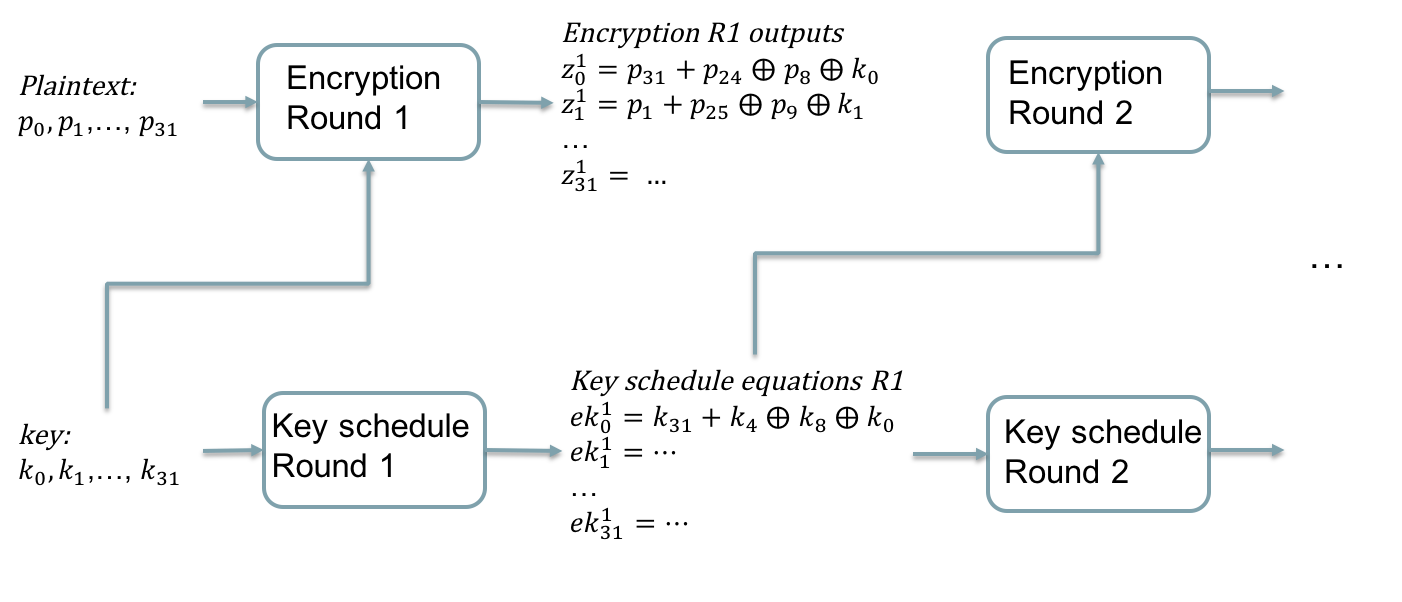
\includegraphics[width=130mm]{./pics/ch3ACmodeling.png}	
	\caption[Toy example for modelling Simon block cipher with a multivariate quadratic equation system]{Toy example for modelling Simon block cipher with a multivariate quadratic equation system. The upper part is the main block encryption with extended keys generated by a key schedule\protect\footnotemark (lower part). }
	\label{fig:ch3ACmodeling}
\end{figure}	
\footnotetext{The key schedule here has a specific recursive form %%%%found
	in popular ciphers such as DES, AES and Simon
	which optimizes storage or chip size and timing.}

% Algerbirc 
In addition, some high profile cryptanalysis problems in public key cryptography can be written in a form that contains a \textit{block cipher topology} \footnote{
	This is basically a property of the equations proposed by Semaev in 2015 \cite{semaev2004summation,cryptoeprint:2015:310}, they have  the same structure as on Figure \ref{fig:blockciphertopology} with variables progressively more and more remote from the constraints which make that the system of equations have a unique solution. The key point is that this sort of configuration leads to a system of equations which is really very hard to solve in the same way as in algebraic attacks on block ciphers.}. Such equations have a similar structure to a block cipher, where the beginning inputs and final outputs variables are easy to get and the middle part of the equation system is very hard to analyse (see Figure \ref{fig:blockciphertopology}). One example is Semaev's summation polynomial equations studied in elliptic curve cryptanalysis \cite{semaev2004summation,cryptoeprint:2015:310} see Section \ref{sec:SemaevCipher}.      

\begin{figure}[h!]
	\centering
	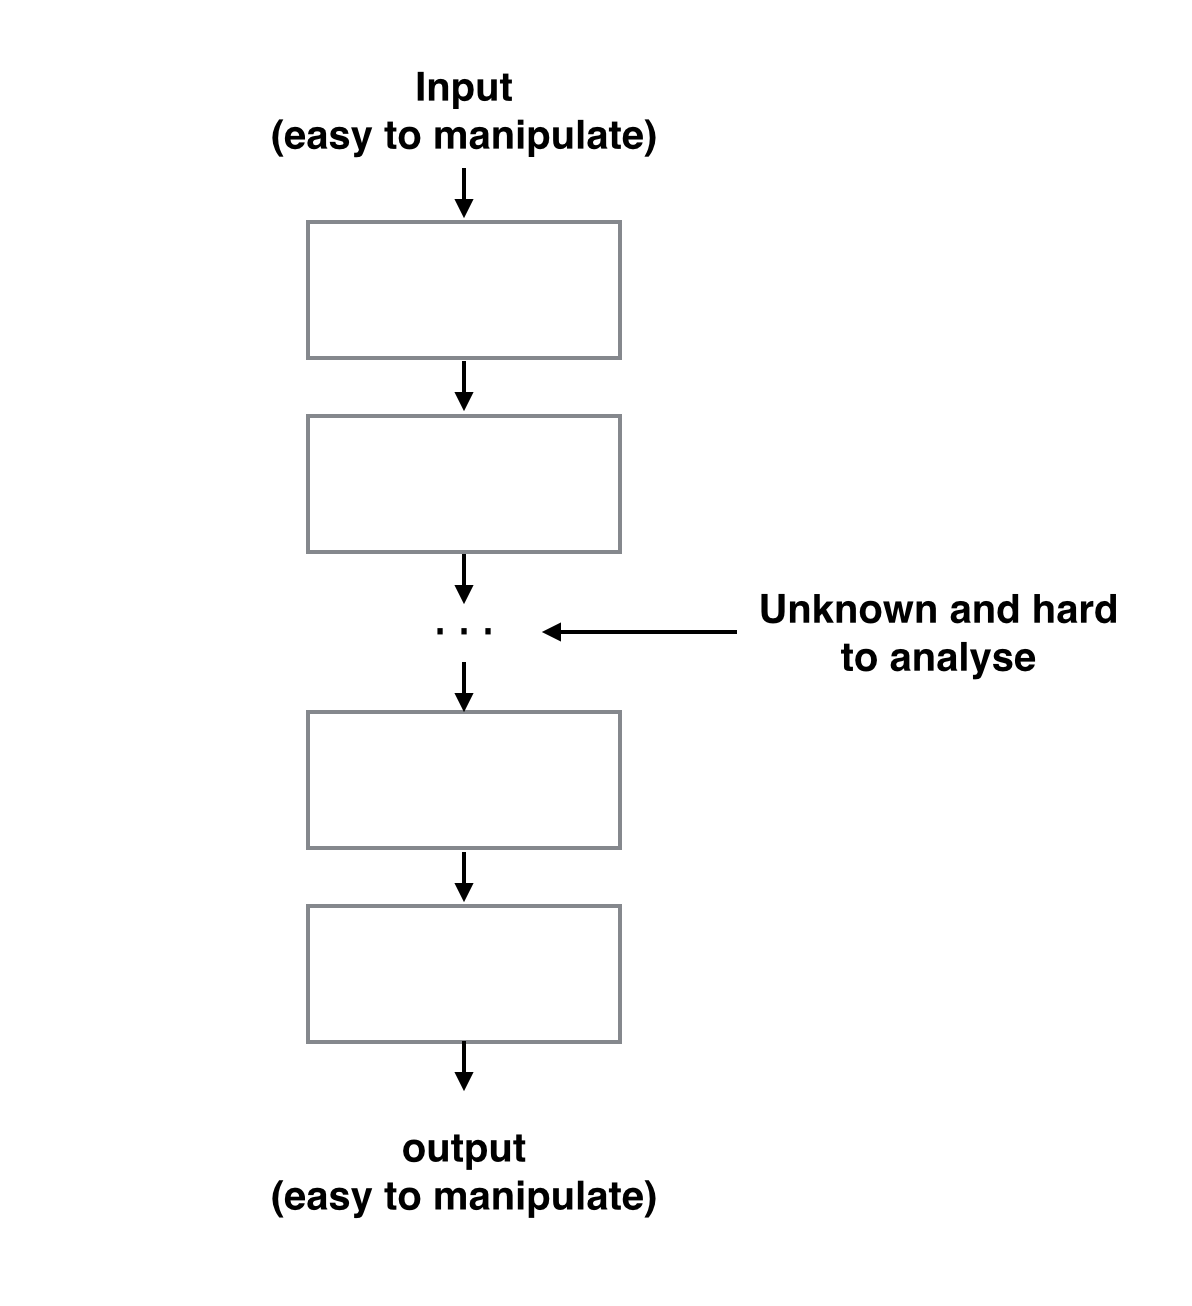
\includegraphics[width=130mm]{./pics/block_cipher_topology2.png}	
	\caption[Block cipher topology] {Block cipher topology: the attacker can control or manipulate
		the inputs and the outputs but it is quite hard to say anything about the variables in the middle}
	\label{fig:blockciphertopology}
\end{figure}	

\subsection{Algebraic Attacks Solving Stage}
Solving a random system of multivariate non-linear boolean equations is an NP-hard problem \cite{fraenkel1980complexity}. As many cryptographic primitives can be described by a sparse multivariate non-linear system of equations over $\mathbb{F}_2$ or any other algebraic systems, several techniques were developed to tackle the problem of solving these equations. A classic approach is to use techniques from algebraic geometry, especially Gr\"{o}bner bases algorithms, to solve the system of equations \cite{faugere1999new}. But most of the time they do not lead to solutions in practice due to the extremely high memory requirements. Subsequently, some heuristic techniques were developed called \textit{linearization} \cite{XL}, where all the non-linear terms are replaced by an independent linear variable and the resulting linear system can be solved using Gaussian elimination \cite{sepehrdad2012statistical}. However, this requires there to be enough linearly independent equations and that the initial system  be highly over-defined and sparse. Then, the XL algorithm \cite{XL,courtois2002cryptanalysis} was developed to make the system over-defined by adding new equations to the current system. The XL proposal made it possible to solve the multi-order non-linear equations within polynomial time, which accelerated the development of the algebraic attacks. Then researchers focused mainly on  fast solutions to the algebraic equation systems. 

Since 2006, Courtois and Bard discovered that this problem could be solved using tools and software \cite{courtois2007algebraicDES}, such as SAT solvers. SAT solvers are automated software solvers which aim to solve one of the original NP-complete problems, the so-called Boolean Satisfiability Problem. 
\begin{mydef} \label{def:booleanSat}[Boolean Satisfiability Problem] 
The SAT problem in Conjunctive Normal Form (CNF) consists of the conjunction ( $\wedge$  representing the Boolean AND connective) of a number of clauses, where a clause is a disjunction ( $\vee$ representing the Boolean OR connective) of a number of propositions or their negations (literals).

If $x_{i}$ represent propositions that can assume only the values True ($\equiv 1 \equiv \top$) or False ($\equiv 0 \equiv \bot$), then an example formula in CNF would be:
$$(x0 \vee x2 \vee x3) \wedge (x3) \wedge (x1 \vee \lnot x2)$$
where $\lnot x_{i}$ is the negation of $x_{i}$.
Given a set of clauses $C_{0}, C_{1}, ... , C_{m-1}$ on the propositions $x_{0}, x_{1}, ... , x_{n-1}$, the problem is to
determine whether the formula $$ F = \bigwedge_{j<m} C_{j}$$ has an assignment of truth values to the propositions such
that it evaluates to True.	
\end{mydef}
In the past decade, the rapid improvements in SAT algorithms has made SAT solvers increasingly popular. Modern SAT solvers have a significant impact on the fields of  electronic design automation, software verification, constraint solving in artificial intelligence, and operations research, among others.  Nicolas Courtois is the pioneer of bringing SAT solvers into action in the area of symmetric cryptanalysis. His paper \cite{bard2007efficient} described how to convert a multivariate quadratic equation system to CNF which can be solved automatically by SAT solvers. The advantage of this technique is that SAT solvers can perform reasonably well and do not require a lot of memory as compared with Gr$\ddot{o}$bner basis-based techniques \cite{grobner}. The only disadvantage is the unpredictability of its complexity. The first algebraic attack on reduced-round block cipher DES was done by Courtois and Bard in 2007 \cite{DEScourtois}. Later in 2008, the first algebraic attack on full block cipher KeeLoq \cite{courtois2008algebraicKeeLoq} took place. In the past 10 years, SAT solvers have been used for attacks on block ciphers, such as GOST \cite{courtois2012contradiction,gostac}, KATAN32 \cite{bard2010algebraic} and the Chinese block cipher SMS4 \cite{erickson2010algebraic},  stream ciphers, such as Crypto-1, HiTag2 and Bivium \cite{soos2009extending,courtois2009practical}, and MiFare Classic smart cards \cite{courtois2008algebraic}.

Another method is to use the ElimLin algorithm \cite{ElimLinR}. ElimLin stands for \textbf{Elim}inate \textbf{Lin}ear, and it is a simple algorithm for solving polynomial systems of multivariate equations over small finite fields. It was initially proposed as a single tool by Courtois to attack DES and CTC/CTC2 ciphers \cite{DEScourtois}. It is also known as the \textit{inter-reduction} step in all major algebra systems. Its main aim is to reveal some hidden linear equations existing in the ideal generated by the system of
polynomials. ElimLin is composed of two sequential stages:

\begin{itemize}
	\item \textbf{Gaussian Elimination:} To discover all the linear equations in the linear span of initial equations.
	\item \textbf{Substitution:} Variables are iteratively eliminated in the whole system based on the linear equations found until no linear equation is left.
\end{itemize}

Given an initial multivariate system of equations over $S^0$ in $\mathbb{F}_2[x_1,x_2,..,x_n]$, then the ElimLin is formally described in algorithm \ref{alg:ElimLin}.

\begin{algorithm} 
	
	\caption{ElimLin Algorithm}
	\begin{algorithmic}\label{alg:ElimLin}
		\STATE \textbf{Input:} $S^0=\{f_1,f_2,...,f_m\} \in \mathbb{F}_2[x_1,x_2,..,x_n]$
		\STATE \textbf{Output:} An updated system of equations $S^T$ and a system of linear equations $S_L$
		\STATE 1. Set $S_L\leftarrow{\O}$ and $S^T \leftarrow S^0$ and $k\leftarrow 1$
		\STATE 2. \textbf{Repeat}
		\STATE For some ordering of equations and monomials perform $Gauss(S^T)$ to eliminate non-linear monomials
		\STATE Set $S_{L'} \leftarrow$ Linear Equations from $Gauss(S^T)$
		\STATE Set $S^T\leftarrow Gauss(S^T)\backslash S_{L'}$
		\FOR {$\forall l \in S_{L'}$, $l$ non-trivial (if l=1and unsolvable then \emph{terminate})} 
		%\STATE Let $l \in S_{L'}$, $l$ non-trivial (if unsolvable then \emph{terminate})
		\STATE Let $x_{i_k}$ be a monomial in $l$
		\STATE Substitute $x_{i_k}$ in $S^T$ and $S_{L'}$ and replace by $l-x_{i_k}$
		\STATE Insert $l$ in $S_L$
		\ENDFOR
		\STATE $k\leftarrow k+1$
	\end{algorithmic}
\end{algorithm}

The study of ElimLin is interesting \cite{ElimLinRevisit,ElimLinUniversalEqs}
precisely because it is simpler to understand than more complex
polynomial algebra techniques \cite{XL,XL2,XLAsEstCourt04,Bardet,DoSemiRegularSequencesExist}. In recent years, ElimLin has been applied to NSA block cipher Simon, LBlock, KATAN32 and PRESENT \cite{courtois2014combined,RaddumSimon,ElimLinUniversalEqs,nakahara2009linear}. The main characteristic of ElimLin is that it quietly dissolves
and makes non-linear equations disappear and generates linear equations. Non-linearity is the main and only thing which makes cryptographic schemes not broken by simple linear algebra. Intuitively, ElimLin seems to work better in cases where there is low non-linearity, since this implies the existence of more linear equations.  Multiplicative complexity (MC) is another notion of non-linearity which was studied in Mourouzis's PhD thesis \cite{TheoPhD} and possibly Elimlin may work sufficiently well in cryptographic primitives with low MC.
However, the complexity of ElimLin attack or software algebraic attacks in general is not well studied. It is not clear why this works and how well the ElimLin attack scales for larger systems of equations. This is a major topic of interest in this thesis.

%

\subsection{Algebraic Complexity Reduction} \label{sec:ACReduction}

In order to break a full cipher, algebraic attacks are normally combined with other cryptanalysis techniques to reduce the solving complexity. This attack scenario consists of two independent tasks: one is how a reduced-round cipher can be solved by software algebraic cryptanalysis which we will discuss in Chapter \ref{ch:GOST}-\ref{ch:ElimLIn}. The other task is called algebraic complexity reduction \cite{gostreport,gostac}, which focuses on how the complexity of solving a full round cipher can be reduced to a problem of breaking a cipher with much fewer rounds. Algebraic complexity reduction raises an important optimization problem in algebraic cryptanalysis: one needs to minimize the costs (regarding the probability that our assumptions hold) and to maximize the benefits (regarding the number and the complexity of interesting relations
which hold under these assumptions).  Amplification which was introduced by Courtois and Debraize in 2008 \cite{AlgSnowCourtoisDebraize} is a notion which occurs in such optimization problems.

\begin{mydef}[Amplification, Informal]
	The goal of the attacker
	is to find a reduction where he makes some assumptions
	at a certain initial cost.
	For example they are true with probability $2^{-X}$
	or work for certain proportion $2^{-Z}$ of keys.
	Then the attacker can in constant time determine
	many other internal bits inside the cipher to the total of $Y$ bits.
	
	We are only interested in cases in which the values
	$X$ and $Z$ are judged realistically for a given attack,
	for example $Z<32$ and $X<128$.
	
	We call amplification the ratio $A=Y/X$.
\end{mydef}

The idea of amplification is to gain additional information inside the cipher with low cost. Amplification is also a general cryptanalysis principle which can apply to many cryptanalysis attacks. For example, a guess-then-determine process can be seen as a form of amplification. With the cost of guessing, attackers gain additional information about the key bits which might lead to knowledge about many other bits inside the cipher. 
Gordon Welchman's diagonal board is also a form of amplification which makes Turing's Bombe machine gain additional information about Enigma encryption settings \cite{CourtoisBlockEnigmaSlides}. 

%Algebraic complexity reduction can be very successful if the cipher has certain special properties. For example, in \cite{gostac}, Courtois found the Russian cipher GOST had many self-similarity properties, which reduced the problem of breaking the full GOST cipher from $2^{64}$ key pairs for 32 rounds to 4 key pairs for 8 rounds and similar results.

%Very little is known about what approach would make an algebraic attack efficient and why.

%phase transition and solving time for random 3 sat problems
%from hard to solve to easy to solve

\section{Cryptanlysis of GOST Block Cipher} \label{sec:introductionToGOST}
The Russian encryption standard
GOST 28147-89 %was developed in the 1970s
is an important government standard
\cite{gost198928147}.
Its large key size of 256 bits makes GOST a plausible alternative for AES-256 and 3-key triple DES.
%% full version maybe %%The latter for the same block size of 64 bits offers keys of only 168 bits.
This indicates that GOST means to be a serious cipher for serious applications
%% full version maybe %%designed with most serious applications in mind.
and at least two sets of GOST S-boxes have been explicitly identified as being used by the most prominent Russian banks, %financial institutions
cf. \cite{schneier2007applied,GOSTRussianReferenceImplementation}.

\subsection{GOST And ISO Standardisation.}
The cost of cryptography is still an important problem for the industry.
For example it was only around 2010 that Intel implemented an encryption algorithm
in some of its CPUs, and nowadays both Intel and AMD have very good support for AES-NI instructions.
It is therefore very important to notice that,
in addition to the very long bit keys,
GOST has a much lower implementation cost
than AES or any other comparable encryption algorithm.
For example, in hardware GOST 256 bits requires less than 800 GE\footnote{GE: (informally) 1 GE is equivalent to 1 AND gate },
while AES-128 requires 3100 GE \cite{PoschmannImplement}.
Thus it is not surprising that GOST became an Internet standard.
It is part of many crypto libraries such as OpenSSL
\cite{GOSTRussianReferenceImplementation}, %,Crypto++},
and is also increasingly popular %and used
outside its country of origin
\cite{PoschmannImplement}.
It is hard to think about a better algorithm for the industry
because of its ultra-low implementation cost and
20 years of cryptanalysis efforts behind it \cite{PoschmannImplement}.
In 2010 GOST was submitted to ISO 18033
to become a worldwide encryption standard.
Less than 10
%Only eight
block ciphers have ever become an
ISO %international
standard.
Unhappily in 2011 several key recovery attacks on GOST were found by researchers
\cite{JapaneseGOSTMITMFSE2011,gostreport,gostac,gostdc0,gostdc2}.

\subsection{Cryptanalysis of GOST} \label{sec:CrytanalysisGOST}
The turning point in the security of GOST was the discovery of the so called
``Reflection'' property described by Kara in Indocrypt 2008 \cite{GOSTReflectionKara}.

The reflection property in GOST is based on its key schedule. GOST is a Feistel cipher with 32 rounds. In each round we have a round function $f_k(X)$ with a 32-bit sub-key which is the original 256-bit key divided into eight 32-bit segments $k = (k_0, k_1, k_2, k_3, k_4, k_5, k_6, k_7)$.
One 32-bit sub-key is used in each round, and their exact order is shown in Table \ref{tab:GOSTKey}:

\begin{table}[!h]
	\centering
	\caption[Key Schedule in GOST]{Key schedule in GOST}
	\label{tab:GOSTKey}
	\addtolength{\tabcolsep}{-6pt}
	\resizebox{\textwidth}{!}{%
		\begin{tabular}{|c|c c c c c c c c|c c c c c c c c|c c c c c c c c|c c c c c c c c|}
			\hline
			rounds &1&&&&&&&8&9&&&&&&&16&17&&&&&&&24&25&&&&&&&32 \\ \hline
			keys & $k_0$ & $k_1$ & $k_2$ & $k_3$ & $k_4$ & $k_5$ & $k_6$ & $k_7$& $k_0$ & $k_1$ & $k_2$ & $k_3$ & $k_4$ & $k_5$ & $k_6$ & $k_7$&
			$k_0$ & $k_1$ & $k_2$ & $k_3$ & $k_4$ & $k_5$ & $k_6$ & $k_7$&
			$k_7$ & $k_6$ & $k_5$ & $k_4$ & $k_3$ & $k_2$ & $k_1$ & $k_0$  \\ \hline
			
	\end{tabular}}
\end{table}

Follow Kara's work in Indocrypt 2008 \cite{GOSTReflectionKara}, we write GOST as the following functional decomposition (to be read from right to left)
$$Enc_{k}=\mathfrak{D}  \circ S \circ \varepsilon \circ \varepsilon \circ \varepsilon$$
where $\varepsilon$ is the first 8 rounds which exploits the whole 256-bit key, $S$ is a swap function which exchanges the left and right hand sides and does not depend on the key, and $\mathfrak{D}$ is the corresponding decryption function with $\varepsilon \circ \mathfrak{D}  = \mathfrak{D} \circ \varepsilon = Id$.

Initially at Indocrypt 2008 only a weak-key attack with time complexity of $2^{192}$ was proposed, with a large proportion of $2^{-32}$ of weak keys. Then in 2011, Courtois propsed an algebraic complex reduction attack which break full 32 rounds GOST using pure algebraic cryptanalysis. 

\begin{myAssumption} \label{AssumptionW}
	\cite{gostreport} Let $A$ be such that $\varepsilon(D) = \overline{D}$ where $D$ is defined as $D=\varepsilon^{3}(A)$.
\end{myAssumption}

\begin{fact}
	\cite{gostreport} Given $2^{64}$ known plaintext there is on average one value $A$ which satisfies Assumption \ref{AssumptionW}. For 63\% of all GOST keys at least one such $A$ exists.
\end{fact}

\begin{fact} 
\cite{gostreport} If $A$ satisfies the Assumption \ref{AssumptionW} and defining $B = \varepsilon(A) $ and $C = \varepsilon(B)$ we have:
\begin{enumerate}
	\item $Enc_k(A) = D$. This is illustrated on the right hand side of Figure \ref{GOSTRef}
	\item $Enc_k(B) = C$. This can be seen on the left hand side of Figure \ref{GOSTRef}
\end{enumerate}
\end{fact}

\begin{figure}[h!] 
	\centering
	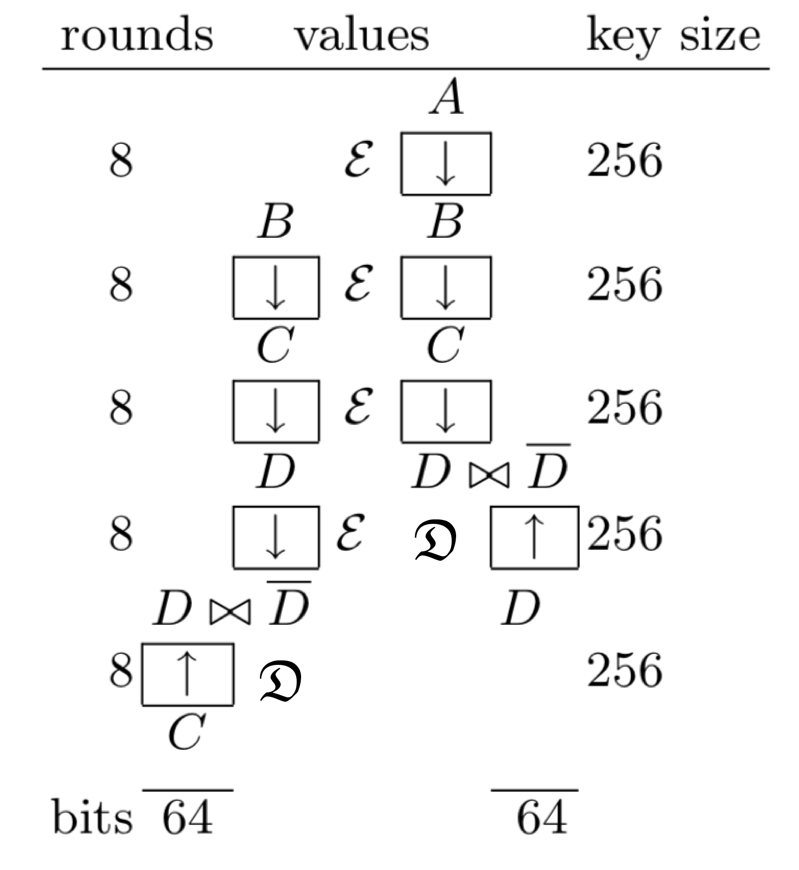
\includegraphics[width=80mm]{./pics/GOSTRef.png}
	
	\caption[Algebraic Complexity Reduction from 32 to 8 rounds of GOST] {Algebraic Complexity Reduction from 32 to 8 rounds of GOST. Due to GOST's self similiarity in the key schedule, the problem of breaking full 32 rounds can be reduced to 8 rounds. The idea is to find 2 Known Plaintext $A$ and $B$ that has properties shown in this figure. }
	\label{GOSTRef}
\end{figure}

\paragraph{From $2^{64}$ KP for 32 Rounds to 4 KP for 8 Rounds:}
Given $2^{64}$ known plaintexts for GOST, it is possible to obtain 4 P/C pairs for 8 rounds of GOST and our guess will be correct with probability $2^{128}$. Thus we obtained 4 pairs for 8 rounds of GOST: $A 􏰀\rightarrow B, B \rightarrow C, C \rightarrow D, D \rightarrow \overline{D}$. As a result breaking 4 P/C pairs 8 rounds of GOST become the last step of breaking full GOST. Courtois said in his papaer the time complexity of breaking 8 rounds GOST is $2^{120}$ \cite{gostreport}. In this thesis we look precisely at questions pertaining to cryptanalysing 8 rounds GOST with less or equal than 4 P/C pairs which can be used as a plugin to replace already known attacks on full GOST.

Many attacks which do not use any reflections
have also been proposed \cite{gostac,gostreport,DunkelmanImprovedGOST8R}
and also differential attacks which do not
fall into the algebraic complexity reduction category.
The most recent advanced differential attack on GOST
has a time complexity of $2^{178}$ \cite{gostdc0,gostdc2}
which is also the best single-key attack known.

\subsection{The Internal Structure of GOST} \label{sec:GOSTStructure}
GOST is a block cipher with a simple Feistel structure,
64-bit block size, 256-bit keys and 32 rounds.
Each round contains a key addition modulo $2^{32}$,
a set of 8 bijective S-boxes on 4 bits,
and a simple rotation by 11 positions.

GOST has 32 identical rounds such as the one described on Figure \ref{GostRoundAndConnections} below.
They differ only by the subsets of 32 key bits which they use. GOST has a weak key schedule which is the main source of all the attacks on full 32-round GOST \cite{gostreport,gostac,JapaneseGOSTMITMFSE2011,gostdcpp1,gostdc0,gostdc1,gostdc2,DunkelmanImprovedGOST8R}.  
In this thesis we only look at up to 8 rounds of GOST which have independent 32-bit keys and don't repeat.

We number the inputs of the S-box Si for $i=1,2,\ldots,8$ by integers from $4i+1$ to $4i+4$ out of $1..32$ and its outputs are numbered according to their final positions after the rotation by 11 positions: for example the inputs of S6 are $21,22,23,24$ and the outputs are $32,1,2,3$.


\begin{figure}[h] 
	\centering
	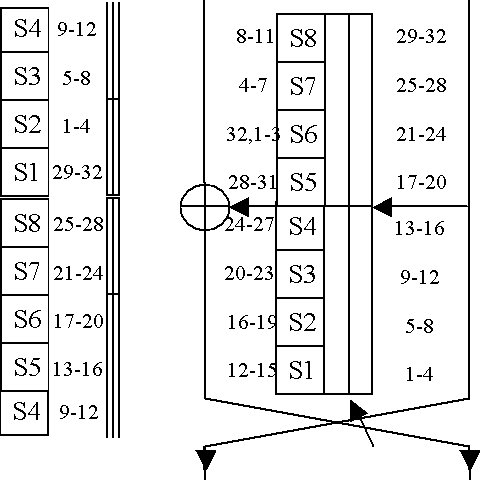
\includegraphics[width=80mm]{./pics/gostfeist2.jpg}
	
	\caption[One Round of GOST And Connections in The Following Round] {One Round of GOST And Connections in The Following Round. This figure describes the encryption process for one round of GOST. Firstly, the 32-bit right half is added with $k_{i}$ (modulo $2^{32}$, showed in figure as  $\boxplus$ ). Then, the result is divided into eight 4-bit consecutive blocks and each block is given as input to a different S-box. The first 4 bits go into the first S-box S1, bits 5-8 go into S2 and so on. Then, the 32-bit output undergoes a 11-bit left circular shift and finally the result is xored to the left 32-bit half of the data.}
	\label{GostRoundAndConnections}
\end{figure}

In Figure \ref{GostRoundAndConnections}
we also show S-box numbers
in the next round in the left margin.
This is very helpful in order to see which bits are successfully determined in our attacks on GOST.
In a great simplification, in most cases, one S-box in one round affects essentially
only two consecutive S-boxes in the next round. Additional propagation is obtained due to the Feistel structure
and due to carries in the modular addition.

\textbf{Modular Addition}: The GOST cipher uses addition modulo $2^{32}$ for key insertion which is another source of introducing non-linearity in the cipher. Here we explain how to algebraically encode modular addition, which is the modelling step of algebraic cryptanalysis. The modular addition of two n-bit words x; y is algebraically
described as follows
\begin{equation}
	(x,y) \mapsto z = x + y \text{ mod } 2^{n}
\end{equation}
The resulting n-bit word $(z_{n-1},...,z_{0})$ is given by:
\[
\left\{
\begin{array}{ll}
z_0 = x_0+y_0\\
z_1 = x_1+y_1+c_1\\
z_2 = x_2+y_2+c_2\\
.\\
z_i=x_i+y_i+c_i \\
.\\
z_{n-1} = x_{n-1} + y_{n-1}+c_{n-1}
\end{array}
\right.
\]
where,
\[
\left\{
\begin{array}{ll}
c_1 = x_0  y_0\\
c_2 = x_1 y_1+c_1(x_1+y_1)\\
.\\
c_i=x_{i-1}y_{i-1}+c_{i-1}(x_{i-1}+y_{i-1})\\
.\\
c_{n-1} = x_{n-2}+y_{n-2}+c_{n-2}(x_{n-2}+y_{n-2}) 
\end{array}
\right.
\]

\section{Cryptanalysis of SIMON Block Cipher}
Nowadays lightweight cryptography is rapidly evolving and becoming more and more important due to the increasing demand from mobile phones and the Internet of Things. These lightweight cryptographic primitives are designed to
be efficient (in both hardware and software) when limited
hardware resources are available and at the same time to
guarantee a desired level of security. The
design of such primitives is a great challenge and can be
seen as a non-trivial optimization problem, where several
trade-offs are taken into account. They need to maintain
a reasonable balance between security and efficient software and hardware
implementation with very low overall cost with respect to several
meaningful metrics (power consumption, energy consumption, size of the circuit \cite{OptimiPaper,BoyarPeraltaMCMethod,BoyarPeraltaMCBoolean}).

The research community has
proposed many lightweight hash functions, block ciphers and stream ciphers which are
reasonably good and satisfy at a reasonable level the trade-off
between efficiency and security. Nowadays, in cryptographic
literature we find lots of such lightweight cryptographic primitives such as
KATAN \cite{KATAN}, KLEIN \cite{KLEIN}, ICEBERG
\cite{ICEBERG}, HIGHT \cite{HIGHT}, LED \cite{LED},
mCrypton \cite{mCrypton}, PRESENT \cite{PRESENT}, Piccolo \cite{Piccolo}
and many others.

In July 2013, a team from the NSA proposed two new families of particularly lightweight block
ciphers, Simon and Speck, both coming in a variety of blocks and key sizes
\cite{NSAciphers}. We have developed a basic reference implementation of both ciphers 
which can be found on Github \cite{simonref},
as well as a generator of algebraic equations to be used in algebraic attacks. 

The designers of Simon and Speck published the full specifications and presented
only performance and implementation footprints, without providing
any advanced security analysis
against known cryptanalytic attacks.
Both of them offer excellent performance on both
hardware and software platforms and perform
exceptionally well across the majority of lightweight applications and
not only on a single platform. Compared to
other lightweight cryptographic primitives,
these two are meant to have better performance with respect to the area
needed for a given throughput, code size and memory usage.
Simon is designed for optimal performance in hardware, and Speck for optimal
performance in software.
According to Aysu's analysis \cite{simoneff}, Simon with an equivalent security level as AES,
is $86\%$ smaller
than AES, $70\%$ smaller than PRESENT and its smallest hardware architecture
only costs 36 slices (72 look-up tables, 30 registers). Recent results about hardware
implementation of block ciphers emphasize reducing the size and/or Multiplicative Complexity (MC) further possibly
leads to optimal implementations \cite{BoyarPeraltaMCMethodAES,OptimiPaper}.

However, in the original NSA paper \cite{NSAciphers}, there is no analysis of the security of these 2 ciphers against major well-known attacks. In the same paper \cite{NSAciphers}, the authors briefly said that Simon and Speck were designed to provide security against traditional adversaries who can adaptively encrypt and decrypt large amounts of data, and some attention was given so that there are no related-key attacks. Except for these comments, no more analysis against common attacks such as linear or differential cryptanalysis was presented and the task of analyzing the resistance of the ciphers against known attacks was left to the academic community. Immediately after the release of the specifications we had the first attempts using differential, linear and rotational cryptanalysis \cite{simon1,simon2}. Our attacks on Simon described in Chapter \ref{ch:SIMON} were the first algebraic cryptanalysis attacks attempted on Simon. The work was published in 2014 \cite{courtois2014combined}. In recent years Simon was studied heavily by a lot of researchers, including differential attacks introduced by Biryukov et al \cite{simon3}, Mourouzis et al \cite{SIMON6} and Wang et al \cite{SIMON4, SIMON5}, also combined differential and linear attacks by Farzaneh et al \cite{simon1} and Alkhzaimi et al \cite{simon2}. Most of them are using statistical cryptanalysis techniques, the best results break around 70\% rounds of different versions of Simon. In 2015, Raddum \cite{raddum2006new} published another algebraic cryptanalysis work on Simon for most of the versions (not including Simon 64/128 version). Raddum's work uses more P/C pairs than our attack and breaks 16 (out of 72) rounds of Simon 128/256 version with ElimLin.  This attack shows that there is a need to understand better how ElimLin attacks can scale to larger attacks. 

\subsection{SIMON Structure}
SIMON is a family of lightweight block ciphers with the aim of havingan  optimal hardware performance \cite{NSAciphers}.
It follows the classical Feistel design paradigm\footnote{Note that in classical Feistel structure computation is done on left side, see \ref{sec:feistel}. In Simon computation is done on right side see Figure \ref{fig:SIMONroundfn}}, operating on two
$n$-bit halves in each round and thus the general block size is $2n$.
The Simon block cipher with an $n$-bit word is denoted by Simon-$2n$, where
$n=16,24,32,48$ or $64$, and if it uses an $m$-word key (equivalently $mn$-bit
key) we denote it as Simon-$2n/mn$. In this chapter, we study the variant of
Simon with $n=32$ and $m=4$ (i.e. 128-bit key).

Each round of Simon applies a non-linear, non-bijective (and as a result
non-invertible) function
\begin{equation}
F:GF(2)^n\rightarrow GF(2)^n
\end{equation}

to the left half of the state which is repeated for 44 rounds.
The operations used are as follows:

\begin{enumerate}
	\item bitwise XOR, $\oplus$
	\item bitwise AND,
	\item left circular shift, $S^j$ by $j$ bits.
\end{enumerate}

We denote the input to the $i$-th round by $L^{i-1}||R^{i-1}$
and in each round the left word $L^{i-1}$ is used as input
to the round function $F$ defined by,

\begin{equation}
F(L^{i-1})=(L^{i-1}<<<1)\wedge(L^{i-1}<<<8)\oplus(L^{i-1}<<<2)
\end{equation}

Then, the next state $L^{i}||R^{i}$ is computed as follows
(cf. Fig. \ref{fig:SIMONroundfn}),

\begin{equation}
L^i=R^{i-1}\oplus F(L^{i-1})\oplus K^{i-1}
\end{equation}
\begin{equation}
R^i=L^{i-1}
\end{equation}


\begin{figure}[!h]
	\vspace{-0.2cm}
	\centering
	%   {\epsfig{file = .\SIMONroundfn.eps, width = 6.5cm}}
	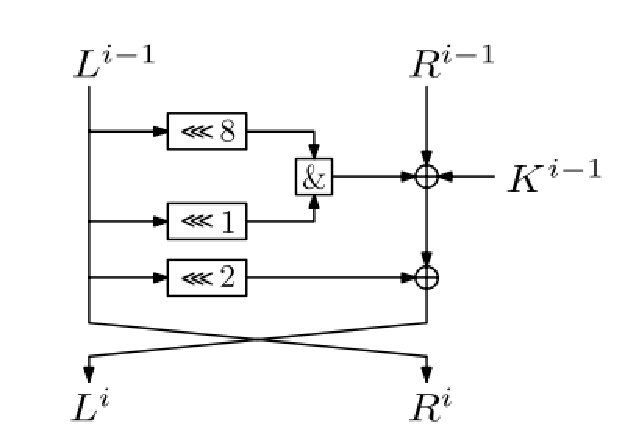
\includegraphics[width=120mm]{./pics/SIMONroundfn-eps-converted-to.pdf}
	\caption{The round function of Simon}
	\label{fig:SIMONroundfn}
	\vspace{-0.1cm}
\end{figure}


The output of the last round is the ciphertext.
\subsection{Key Schedule}
The key schedule of Simon is based on an Linear-Feedback Shift Register(LSFR)-like procedure \cite{lindell2014introduction}, where the $nm$-bits of the key are used to generate the keys $K_0,K_1,...,K_{r-1}$ to be used in each round. There are three different key schedule procedures depending on the number of words that the secret key consists of ($m=2,3,4$).

At the beginning, the first $m$ words $K^0,K^1,...,K^{m-1}$ are initialized with the secret key, while the remaining are generated by the LSFR-like construction. For the variant of  interest, where $m=4$, the remaining keys are generated in the following way:
\begin{equation}
Y=K^{i+1}\oplus (K^{i+3}>>>3)
\end{equation}
\begin{equation}
K^{i+4}=K^i\oplus Y \oplus (Y>>>1)\oplus c\oplus (z_j)_i
\end{equation}

The constant $c=0xff...fc$ is used for preventing slide attacks and attacks exploiting rotational symmetries \cite{NSAciphers}. In addition, the generated subkeys are XORed with a bit $(z_j)_i$, that denotes the $i$-th bit from the one of the five constant sequences $z_0,...,z_4$. These sequences are defined in the NSA's orginial paper \cite{NSAciphers} and for our variant we use $z_3$. We have implemented a basic reference implementation of Simon and Speck ciphers and a basic generator of equations that are used in algebraic attacks \cite{simonref} .

The Feistel network, the construction of the round function and the key generation of Simon, enables bit-serial hardware architectures which can significantly reduce the cost of implementation \cite{simoneff}. Additionally, encryption and decryption can be done using the
same hardware.

\section{Summary} \label{sec:ACCxty}
Algebraic cryptanalysis attacks allow the cryptanalyst to recover secret key bits given only one or very few plaintext / ciphertext pairs. However, one of the fundamental problems of algebraic cryptanalysis is that the runtime of algebraic attacks against block ciphers is not well understood. In 2007, Courtois and Bard said in the first paper describing an algebraic attack on block cipher \cite{DEScourtois}:

\begin{quotation}
	``Very little is known about what approach would make an algebraic attack efficient and why." 
\end{quotation}


Up to today, this question still remains in algebraic cryptanalysis. At the moment most of the exising Algebraic Cryptanalysis applications are just coverting target ciphers to equation systems and then solved directly by a software solver  (i.e ElimLin or SAT solvers). Very limited research has been done in order to understand the behavior of a solver and how to make the coverted equation system become easier to solve. 

On cryptanalysis of block ciphers we introduced two well known encryption standards: Russian GOST and NSA SIMON. We reviewed the state of art cryptanalysis works on these encryption standards: best algebraic cryptanalysis attack on 8 rounds GOST require time complexity of $2^{120}$ and no algebraic cryptanalysis has been done on SIMON. The above facts motivate our research work decribed in Part \ref{Part2} of the thesis. 

In Chapter \ref{ch:GOST} we will introduce a fundemental notion of ``contradiction immunity`` and describe how conradiction can be used in algebraic cryptanalysis. We will demostrate a mixed SAT/UNSAT attack on GOST which improve the time complexity of current best attack on breaking 8 rounds of GOST from $2^{120}$ to $2^{92}$. In Chapter \ref{ch:SIMON} we will describe a new Algebraic Cryptanalysis approach combined with well selected P/C paris in a Chosen Plaintext Attack scenario and benchmark our attacks with randomly selected P/C pairs. We will apply this method in newly proposed NSA cipher SIMON and provide the first Algebraic Cryptanalysis on SIMON block cipher. Finally in Chapter \ref{ch:ElimLIn} we will study the behavior of ElimLin method with regards to the number of data samples availiable to an attacker. By studying the number of linear independent equations found by ElimLin, we will show ElimLin has a phase transition process where the number of equations found by ElimLin increase much faster than linear and eventually break the cipher. We will then inspect where the faster than linear groth come from and study how to find more equations that ElimLin can not yet find.


\chapter{Conclusion}
\label{chapterlabel4}

This thesis mainly focuses on improving algebraic cryptanalysis with software and solvers. Algebraic cryptanalysis is powerful as it requires small quantities of data, but in general the complexity grows quickly as the number of rounds increases. Many mitigations to improve runtimes are studied. 
We explored different types of optimization processes meant to make algebraic cryptanalysis problems transition from ``hard to solve" to ``easier to solve" by a software solver. We applied these optimizations to concrete ciphers and demonstrated the improvements. We aim to contribute to future government standards, such as Simon and other widely used ciphers including new releases of GOST.  We proposed several possible optimizations for algebraic cryptanalysis and experimentally demonstrated the attacks on GOST and Simon, which were submitted to ISO. We explore many powerful enhancements for algebraic attacks, and in one case we show a result which upper bounds can be obtained, and suggest a new method to predict the complexity of future attacks. 
We also propose an optimized attack for Bitcoin brain wallet attack.  

In Chapter 4, we introduced a new notion of contradiction immunity and SAT immunity, which converts a first stage in cryptanalysis of GOST to an optimization problem. Then we implemented a guess-then-solve attack with a well chosen set of guessed bits. This attack later directly improved the current best attack on GOST. Incidentally GOST was rejected by ISO at that time. 

In Chapters 5-6 we studied NSA block cipher Simon which was introduced in 2013 and submitted to ISO in 2015. 
We introduced a new method that uses well selected P/C pairs which follow a truncated differential property for algebraic cryptanalysis, and demonstrated the improvement on basic algebraic attacks on Simon with an extremely detailed study of what happens inside the attack and a serious improvement which generates more equations directly. Our work breaks 10/48 rounds of Simon64/128 with less than 10 P/C pairs.
We disagree when some researchers believe that Simon should not be studied by academics: 

\begin{quotation}
	``%`SIMON and SPECK should not even be reviewed by anyone in the community, 
	because it dignifies [the designs] and wastes the cycles – the brain cycles – of intelligent people, by going to look at a thing that is produced by a bad actor agency [(the NSA)]." \\ 
\rightline{{--- Jacob Appelbaum, FSE 2015 invited talk \phantom{This ble} }}
\end{quotation}

We propose an opposite view: it is important for the research community to study Simon because it is likely to become an important industry standard in the future. We published the first algebraic cryptanalysis work on Simon in 2014. Today, it is not the best attack. But it is important for the community to notice Simon's low multipicative complexity, low non-linearity and its low security against algebraic cryptanalysis which is also shown 
in Section \ref{Sec:ElimLinVsApprox}. 

In our research we spent a lot of time on contemplating what happens inside ElimLin algorithm. It contains a rich variety of attacks, for example, various generalizations of cube attacks not previously studied. 
ElimLin is a powerful tool for algebraic cryptanalysis, but with a fundamental limitation on computational complexity. When trying to solve larger number of rounds, the converted problems get much more bigger and ElimLin can not provide an answer within a short time. With a large number of experiments using ElimLin on Simon, we show that precise prediction for ElimLin is possible. We have made progress in both understanding better and extending/enhancing the ElimLin attack. Our discovery method 
of Section \ref{Sec:ElimLinVsApprox} suggests that the same equations can yet be computed a lot more efficiently. 

Finally, we also looked at the widely used cryptography application --  ECDSA in Bitcoin with the secp256k1 curve in Chapter 7. Elliptic curve problems themselves are hard algebraic cryptanalysis problems with complex polynomials and sometimes equations which follow the same topology as in a block cipher. Here nobody is yet able to 
propose advanced practical attacks. Another application we studied is Bitcoin. 
It was invented in 2008 and has grown rapidly since 2012, and it's one of the largest ECC practical applications in the world. We studied how some users manage their private keys and the security pitfalls related to this. Bitcoin uses a special elliptic curve secp256k1 which has not been widely used by any previous application, and in this thesis we provide a detailed benchmark of all the major implementations of this curve, and propose an optimized password cracking attack on Bitcoin brain wallets with a slightly unusual ECC  speed optimization. Our work together with other researchers work had made the Bitcoin community aware that brain wallets are extremely insecure.  
% This just dumps some pseudolatin in so you can see some text in place. 


\addcontentsline{toc}{chapter}{Appendices}

% The \appendix command resets the chapter counter, and changes the chapter numbering scheme to capital letters.
%\chapter{Appendices}
\appendix
\chapter{An Appendix About Stuff}
\label{appendixlabel1}
(stuff)

\chapter{Another Appendix About Things}
\label{appendixlabel2}
(things)

\chapter{Colophon}
\label{appendixlabel3}
\textit{This is a description of the tools you used to make your thesis. It helps people make future documents, reminds you, and looks good.}

\textit{(example)} This document was set in the Times Roman typeface using \LaTeX\ and Bib\TeX , composed with a text editor. 
 % description of document, e.g. type faces, TeX used, TeXmaker, packages and things used for figures. Like a computational details section.
% e.g. http://tex.stackexchange.com/questions/63468/what-is-best-way-to-mention-that-a-document-has-been-typeset-with-tex#63503

% Side note:
%http://tex.stackexchange.com/questions/1319/showcase-of-beautiful-typography-done-in-tex-friends 
% You could separate these out into different files if you have
%  particularly large appendices.

% This line manually adds the Bibliography to the table of contents.
% The fact that \include is the last thing before this ensures that it
% is on a clear page, and adding it like this means that it doesn't
% get a chapter or appendix number.
\addcontentsline{toc}{chapter}{Bibliography}

% Actually generates your bibliography.
\bibliography{example}

% All done. \o/
\end{document}
